\documentclass[11pt]{article}
\usepackage{fullpage,amsmath,amsfonts,mathpazo,microtype,nicefrac,graphicx,verbatimbox,hyperref,listings,enumitem,amssymb,float,fancyhdr}
\newcommand{\na}{$\emptyset$}
\newcommand{\modZ}[1]{$\mathbb{Z}_{#1}$}
\hypersetup{
  colorlinks = true
}

\title{
\vspace{1cm}
\textmd{\textbf{AM205 Final Project: Modulo-n Lights Out}}\\
}

\author{\textbf{Shawn Pan and Andrew Ross}}
\date{\today}

%----------------------------------------------------------------------------------------

\begin{document}

\maketitle

\section*{Introduction}

\paragraph{} Lights Out is an electronic puzzle game released by Tiger Electronics (who notably also developed the \href{https://en.wikipedia.org/wiki/Furby}{Furby}) in 1995. An individual puzzle in Lights Out consists of a configuration of lit and unlit buttons on a 5x5 grid. Pressing any button toggles its state and that of the four adjacent buttons, and the goal is to turn all lights off in as few moves as possible.

\paragraph{} The effect of any sequence of presses can be represented as a modulo 2 sum of vectors (where each 2D board coordinate is mapped to a 1D vector position), and because summation is commutative, the sequence of presses will have the same effect regardless of its order. We can represent the constraints of the problem as a system of equations in $\mathbb{Z}_2$ (i.e. modular arithmetic on $\{0, 1\}$), which we can more helpfully write as a matrix equation

\begin{equation}
Ax = b,
\end{equation}

\noindent where $b = \langle g_{11}, g_{12}, \cdots, g_{15}, g_{21}, \cdots, g_{55} \rangle$ is the length-25 vector of grid states $g_{ij}$, which are 1 if lit and 0 otherwise, $x$ is the length-25 vector of presses, and $A$ is a matrix that encodes the transitions. In the standard Lights Out game, $A_{ij}$ is 1 along the main diagonal and, except at 2D board edges, 1 at positions one and five cells above and below the main diagonal. In the more general case, $A$ can be any matrix encoding transitions, the grid can have any dimensions, and transitions can occur not just in $\mathbb{Z}_2$ (modulo 2) but $\mathbb{Z}_k$.

\paragraph{} There are many ways to solve this matrix equation; in the case that $A$ is invertible, we can find its inverse $A^{-1}$ and obtain a unique solution $x = A^{-1}b$. Alternatively, we can use a factorization technique such as the LU decomposition to find $x$ more efficiently. In the case that $A$ isn't invertible, then in general it is possible that there may not be any $x$ such that $Ax = b$, and if there is, then $x$ will no longer be unique (although the shortest $x$, i.e. the $x$ that minimizes $\sum x_i$, may still be).

\paragraph{} \cite{jaap} provides a great analysis of the core mathematics of the game and several variants. In particular, \cite{jaap} devotes a significant amount of time to generalizing board dimensions, with some limited discussion of the game in $\mathbb{Z}_3$, which was released as Lights Out 2000. \cite{giffen} and \cite{involve} approach the problem from the perspective of graph theory and graph coloring problems, generalizing it to arbitrary transition matrices in $\mathbb{Z}_k$. A particular focus of \cite{giffen} and \cite{involve} is determining when the game is always winnable, and on methods of generating families of transition graphs with certain properties.

\paragraph{} Our goal is to reproduce and generalize results from \cite{jaap} and confirm they agree with theorems presented in \cite{giffen} and \cite{involve}. We also want to demonstrate a software package we wrote for solving modular systems of equations and visualizing solutions to Lights Out puzzles.

\paragraph{} Additionally, since solutions to light puzzles (arrays of press patterns) can also be interepreted as grids, we consider the recursive problem of solving a grid, then solving its solution, and so on, until we reach a state we have already seen or one that cannot be solved. The simplest version of this (a complete cycle of length 1) corresponds exactly to eigenvectors of the transition matrix with eigenvalue 1. We will explore these cycles of solutions and attempt to relate them to the theoretical work in \cite{jaap}, \cite{giffen}, and \cite{involve}.

\section*{Nullity and Solvability}

\paragraph{} As we noted above, when $A$ is invertible, then we can solve the puzzle uniquely for any initial board configuration $b$. When $A$ isn't, we are interested in the dimension of its nullspace. In particular, if the nullspace of $A$ is $d$-dimensional, then there will be $d$ linearly independent press patterns that have no effect on the board. These are referred to as "quiet patterns" in \cite{jaap}, and a basis for them can be determined by augmenting $A$ with the identity matrix and performing Gaussian elimination to transform $A$ as close to the identity as possible.

\begin{figure}
\caption{Plots of the dimension of the nullspace of the standard Lights Out transition matrix at various grid sizes and moduli}
\label{nullity}
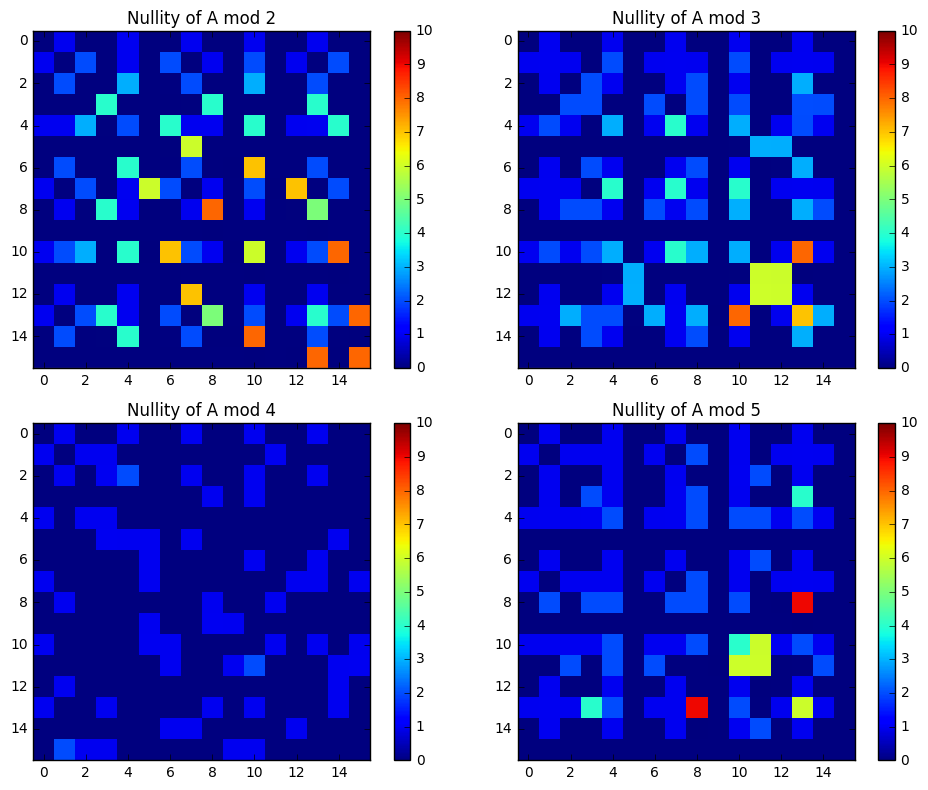
\includegraphics[width=\textwidth]{nullity.png}
\end{figure}

\paragraph{} The dimension of the nullspace can also be determined by performing modulo-$k$ LU factorization on $A$, then counting the number of nonzero entries in the upper-triangular matrix $U$, which is how we calculate it in practice. We do this in Figure \ref{nullity}, which agrees with the tables of results shown in \cite{jaap} for $k=2$ and $k=3$, but generalizes them up to $k=13$.

\begin{figure}
\caption{Plots of theoretical predictions for solvability based on \cite{involve}  The relatively prime entries are in blue.}
\label{relprime}
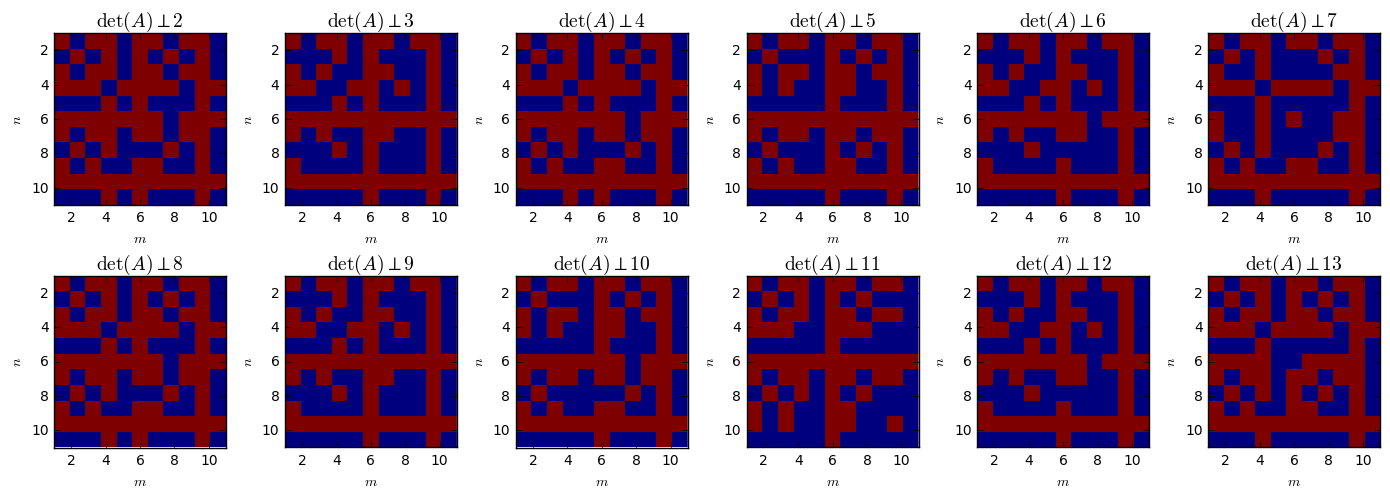
\includegraphics[width=\textwidth]{relprime.png}
\end{figure}

\paragraph{} What's interesting, though, is that our plots in Figure \ref{nullity} actually disagree in certain cases with a theoretical result from \cite{involve}, which states that $A$ must span $\mathbb{Z}_k$ if $det(A)$ and $k$ are coprime (i.e. their greatest common denominator is 1). Figure \ref{relprime} shows plot of those theoretical predictions, which you can see agree with the results in Figure \ref{nullity} but only when $k$ is prime. Coincidentally, \cite{involve} only proves that result for prime values of $k$, but it is unclear whether their result actually doesn't hold for non-prime values of $k$ (or if there is an error in our code).

\begin{figure}
\caption{Comparison of full rank grid sizes for the standard transition matrix for mod 2, mod 3, and mod 6}
\label{overlap236}
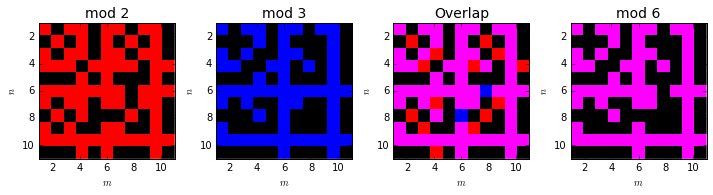
\includegraphics[width=\textwidth]{mod6overlap.png}
\end{figure}


\section*{Solving Matrices on a Modular Field}

\subsection*{LU Factorization}

\paragraph{} We have implemented a variant of LU factorization to efficiently solve our transition matrices over a modular field.  The standard LU factorization decomposes the matrix into a product of a lower diagonal matrix $L$ and an upper diagonal matrix $U$.  The decomposed form allows problems of the form $Ax = b$ to be solved efficiently chaining 2 triangular matrix solves.  Triangular matrices can be solved with forward and backward substitution.


\paragraph{} Since the standard LU algorithm is well known, we will focus our attention on the details for implementing it over a modular field.  Addition, subtraction, and multiplication can all be carried on as usual with an additional modulo step at the end to keep the result in the valid range.  The major challenge of LU factorization over a modular field that we faced was handling division.  Division should be treated as the inverse of multiplication.  For example $3 / 2 = 4$ in mod 5, because $2 \times 4 = 3$.  Because we explored relatively small moduli, we precomputed the appropriate division tables by looping over all the pairwise multiplications.


\subsection*{Partial Pivoting}

\paragraph{} The default LU algorithm quickly runs into issues with zero diagonal entries.  Division by zero is undefined during the elimination step.  The standard solution to deal with zero entries and to improve numerical accuracy is partial pivoting.  Rows are swapped to bring the largest remaining element to the active row, and the final factorization become $PA = LU$ where $P$ is a permutation matrix for the rows.  Because all our arithmetic is performed exactly over a finite field, we don’t particularly care about getting the largest element for numerical stability.  Instead, we just want to get rid of the zero entry on the diagonal.


\paragraph{} A naive first attempt is to swap a row with zero diagonal entry with any row containing a non-zero entry in the corresponding spot.  This method works perfectly well for a prime modulus, but we run into issues with composite moduli.  For example, consider $1 / 2$ mod 6.  There is no solution satisfying $2x = 1$ in mod 6.  This undefined division becomes a problem if 2 is a diagonal entry.  Therefore, we require that the pivots values for the diagonal be relatively prime to the modulus.


\paragraph{} As a second pass, we use partial pivoting to select a row to make the diagonal entry relatively prime to the modulus.  We implemented Euclid’s algorithm to find the greatest common factor.  It turns out that this solution works when the modulus is prime or a power of a prime.  The solution solves many matrices with other composite moduli, but runs into some issues.  Consider the following example of an invertible matrix in mod 6:

\[
A =
\begin{pmatrix}
2 & 3 & 0 \\
3 & 1 & 1 \\
3 & 0 & 2
\end{pmatrix}
\quad
A^{-1} =
\begin{pmatrix}
2 & 0 & 3 \\
3 & 4 & 4 \\
3 & 3 & 5
\end{pmatrix}
\]

\paragraph{} 1 and 5 are the possible pivot factors which are relatively prime to 6.  None of the entries in the first column of $A$ are suitable as pivot factors.  Intuitively, the problem is that none of rows are suitable for pivoting, but the matrix is not singular because a linear combination of 2 rows is a valid pivot: $2 + 3 = 5$.  There are however a couple entries of 1 in the middle column.

\subsection*{Full Pivoting}

\paragraph{} We next implemented full pivoting to get more choices for possibly pivot factors.  With full pivoting, columns may also be swapped.  The factorization then becomes $PAQ = LU$ where $P$ and $Q$ are the row and column permutation matrices respectively.  In the previous example, full pivoting allows use to move the 1 in the center of the matrix to the active diagonal spot for factorization.  Although full pivoting work is sufficient for over 90\% of the cases we explored, occasionally it still fails to solve an invertible matrix, such as the following matrix in mod 6:

\[
A = A^{-1} =
\begin{pmatrix}
4 & 3 \\
3 & 4
\end{pmatrix}
\]

\subsection*{Checking for Linear Combinations}

\paragraph{} To deal with the matrix above, we need to check for linear combinations of rows and columns that may create suitable pivot values.  In our example, $4 + 3 = 1$ mod 6, so adding the two rows will make the matrix solvable.  Systematically checking all the linear combinations is complex and computationally expensive, as the direct approach is exponential with the number of remaining rows.  We instead take a stochastic approach and add 100 random rows in an attempt to create a linear combination with a suitable pivot.  If no suitable pivot is found, we treat the matrix as singular.  In practice this approach solved all the matrices we tried for our experiments.  It may be interesting future work to look into efficient deterministic ways to determine the correct linear combination of rows to take.


\paragraph{} It is somewhat surprising that full pivoting alone is not sufficient to solve all non-singular matrices.  An interesting side effect of taking linear combinations of rows is that the row permutation matrix $P$ is no longer strictly a permutation matrix.  $P$ may include extra values representing the linear combinations taken.

\section*{Singular Transition Matrices}

\paragraph{} Although LU factorization followed by forward and backward substitution works well for solving full rank matrices, the default procedure does not work for singular matrices.  When exploring the light out problem, we often run into this issue.  For example, consider the transition matrix for the standard 5x5 lights out game.  The matrix has rank 23 and nullity 2.  The interpretation is that not all states in the game are reachable from a blank grid.  The game has a solution space of $2^23$ states and null space of $2^2$ states.  We have adapted our algorithm to deal with the singular cases with multiple solutions for a prime modulus.

\subsection*{Multiple Solutions for Prime Modulus}

\paragraph{} The rank of the matrix is equal to the number of non-zero entries along the upper diagonal factor $U$.  Therefore, we may proceed as usual with the standard LU algorithm until the backward substitution step.  In the backward substitution step, we will run into $n$ zero diagonal entries, where $n$ is the nullity of the original matrix.  These zero diagonal entries correspond to equations of the form $0x = 0$ or $0x = 1$.  In the $0x = 1$ case, the system is inconsistent and has no solutions.  In the $0x = 0$, the system has multiple solutions, because we essentially have an unconstrained free parameter.


\paragraph{} Let $z_1, z_2, \dots, z_n$ be the indices for the singular diagonal entries, i.e. $U_{z_i, z_i} = 0$.  We can change the matrix to be no longer singular by setting $U_{z_i, z_i} = 1$, essentially adding an extra equation to the system.  We do not have any constraint on $x_{z_i}$ and can set it to any of value from 0 to $m - 1$ for a field with prime modulus $m$.  We consider 3 different ways to picking the free parameter $x_{z_i}$.  Our solve method implementation takes in a flag for which method to use.

\begin{itemize}
\item Any: We pick all $x_{z_i}$ to be 0, which will return an arbitrary solution.
\item Basis: For each of the $n$ zero diagonal entries, we perform a reverse solve with a single $x_{z_i}$ set to 1 and all other free parameters $x_{z_j} \> (j \ne i)$ set to 0.  This procedure finds $n$ solutions which form a basis for the nullspace.
\item All: For each of the $m^n$ possible free parameter choices for $x_{z_i}$, we perform a reverse solve.  This procedure finds all possible solutions to the equation.  The number of solutions grows exponentially with the dimensions of the nullspace.
\end{itemize}

\subsection*{Applications of Finding Multiple Solutions}

Applications of finding multiple solutions of a singular matrix include finding eigenvalues and quiet states.


The 5x5 cases has a nullity of 2.

\begin{figure}
\caption{Plots of all quiet states for the standard 5x5 game.  Agrees with results from \cite{jaap}}
\label{quiet55}
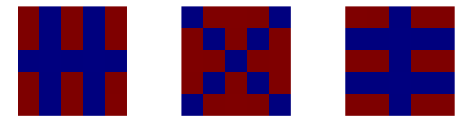
\includegraphics[width=4in]{quiet55.png}
\end{figure}


We can find eigenvectors of eigenvalue $\lambda$ by solving the singular matrix $A - \lambda I$.  For the 7x7 mod 2 case, we find 7 linearly independent eigenvectors.

\begin{figure}
\caption{Plots of the 7 basis eigenvectors of the standard 7x7 game.}
\label{eigbasis77}
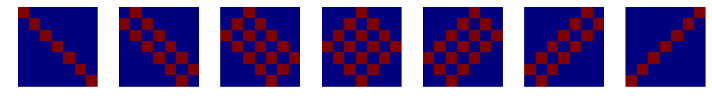
\includegraphics[width=\textwidth]{eigbasis77.png}
\end{figure}


\subsection*{Challenges with Composite Modulus}

\paragraph{} We briefly explored finding solutions to singular matrices over fields with composite moduli.  The rank of a matrix would now be the number of relatively prime diagonal entries in $U$.  A major challenge is that not all singular values are equivalent, and we have a wide variety of cases beyond $0x = 0$ and $0x =1$.  For example, in mod 6 you can have rows representing equations such as $3x = 0$ which has 3 solutions of 0, 2, and 4, or $2x = 1$ which has no solution.  Even to correctly count the number of solutions is challenging and depends on the particular non-relatively prime values along the diagonal.  Enumerating all the solutions for the composite case may be interesting future work.

\section*{Eigengrids and Solution Cycles}

\paragraph{} Eigengrids (with eigenvalue 1) are characterized by the following equation:

\begin{equation}
Ax = x,
\end{equation}

\noindent and repeating solution "cycles" (of period $n$) are characterized by:

\begin{equation}
A^nx = x,
\end{equation}

\noindent or in other words, $x$ is an eigengrid of $A^n$. For every non-singular $A$ (at least using the standard Lights Out transition matrix), we found that $A^n$ actually always equalled the identity matrix for some $n$ (although there would still be a spectrum of eigenstates of lower powers of $A$).

\paragraph{} For singular matrices $A$, we also found cases where

\begin{equation}
\begin{split}
  A^{n_1 + n_2}x & = A^{n_1}x,\\
  A^{n}x & \neq x \text{ for all } n,
\end{split}
\label{eq:transient}
\end{equation}

\noindent that is, where after $n_1$ "iterations" of solving solutions, we would enter a repeating solution cycle with period $n_2$ that didn't contain our initial set of $n_1$ transient states. In these cases $A^n$ never equalled the identity, which clearly must be true for \eqref{eq:transient} to hold.

\begin{figure}
  \caption{Counts of eigenstates of $A^n$ for $2 \times 2$ and $3 \times 3$ grids at various \modZ{k}}
  \label{eigencounts}

  \begin{center}
  \begin{tabular}{|l|l|l|l|l|l|l|}
    \hline
    \multicolumn{7}{|c|}{\# Eigenstates of $A^n$ for $2 \times 2$ grid} \\ \hline
    $k, n$&\textbf{1}&\textbf{2}&\textbf{4}&\textbf{6}&\textbf{8}&\textbf{Total}\\ \hline
    \textbf{2}  & 4   & 12   & 0    & 0    & 0    & $16=2^4$ \\ \hline
    \textbf{3}  & 9   & 18   & 0    & 0    & 0    & $36$ \\ \hline
    \textbf{4}  & 16  & 112  & 128  & 0    & 0    & $256=4^4$ \\ \hline
    \textbf{5}  & 25  & 100  & 500  & 0    & 0    & $625=5^4$ \\ \hline
    \textbf{6}  & 36  & 396  & 0    & 0    & 0    & $432$ \\ \hline
    \textbf{7}  & 49  & 294  & 0    & 2058 & 0    & $2401=7^4$ \\ \hline
    \textbf{8}  & 64  & 960  & 1024 & 0    & 2048 & $4096=8^4$ \\ \hline
    \textbf{9}  & 81  & 648  & 0    & 0    & 0    & $729$ \\ \hline
    \textbf{10} & 100 & 1900 & 8000 & 0    & 0    & $10000=10^4$ \\ \hline
  \end{tabular}
  \vspace{0.5cm}

  \begin{tabular}{|l|l|l|l|l|l|l|l|}
    \hline
    \multicolumn{8}{|c|}{\# Eigenstates of $A^n$ for $3 \times 3$ grid} \\ \hline
    $k, n$&\textbf{1}&\textbf{2}&\textbf{4}&\textbf{8}&\textbf{12}&\textbf{24}&\textbf{Total}\\ \hline
    \textbf{2}  & 8   & 24   & 480    & 0      & 0     & 0       & $512=2^9$ \\ \hline
    \textbf{3}  & 27  & 0    & 0      & 19656  & 0     & 0       & $19683=3^9$ \\ \hline
    \textbf{4}  & 64  & 960  & 130048 & 131072 & 0     & 0       & $262144=4^9$ \\ \hline
    \textbf{5}  & 125 & 0    & 0      & 0      & 78000 & 1875000 & $1953125=5^9$ \\ \hline
  \end{tabular}
  \end{center}
\end{figure}

\begin{figure}
  \caption{Degree to which $A$ is a root of the identity for \modZ{2} and \modZ{3} at various grid sizes}
  \label{cycles-table}
  \begin{center}
  \begin{tabular}{|l|l|l|l|l|l|l|}
    \hline
    \multicolumn{7}{|c|}{Identity Root for $A$ in $\mathbb{Z}_2$} \\ \hline
    $n\times m$&\textbf{2}&\textbf{3}&\textbf{4}&\textbf{5}&\textbf{6}&\textbf{7}\\ \hline
    \textbf{2} & 2   & & & & & \\ \hline
    \textbf{3} & \na & 4   & & & & \\ \hline
    \textbf{4} & 6   & 12  & \na & & & \\ \hline
    \textbf{5} & \na & \na & 12  & \na & & \\ \hline
    \textbf{6} & 14  & 28  & 126 & 28  & 14 & \\ \hline
    \textbf{7} & \na & 8   & 24  & \na & 56 & 8 \\ \hline
  \end{tabular} \begin{tabular}{|l|l|l|l|l|l|l|}
    \hline
    \multicolumn{7}{|c|}{Identity Root for $A$ in $\mathbb{Z}_3$} \\ \hline
    $n\times m$&\textbf{2}&\textbf{3}&\textbf{4}&\textbf{5}&\textbf{6}&\textbf{7}\\ \hline
    \textbf{2} & \na & & & & & \\ \hline
    \textbf{3} & \na & 8   & & & & \\ \hline
    \textbf{4} & 8   & \na & \na & & & \\ \hline
    \textbf{5} & \na & \na & 24  & \na & & \\ \hline
    \textbf{6} & 26  & 728 & 728 & 78  & 26  & \\ \hline
    \textbf{7} & \na & 80  & \na  & \na & \na & 80 \\ \hline
  \end{tabular}
  \end{center}
\end{figure}

\begin{figure}
  \caption{Nullity and degree to which $A$ is a root of the identity at various $\mathbb{Z}_k$ and grid sizes}
  \label{cycles-vs-null}
  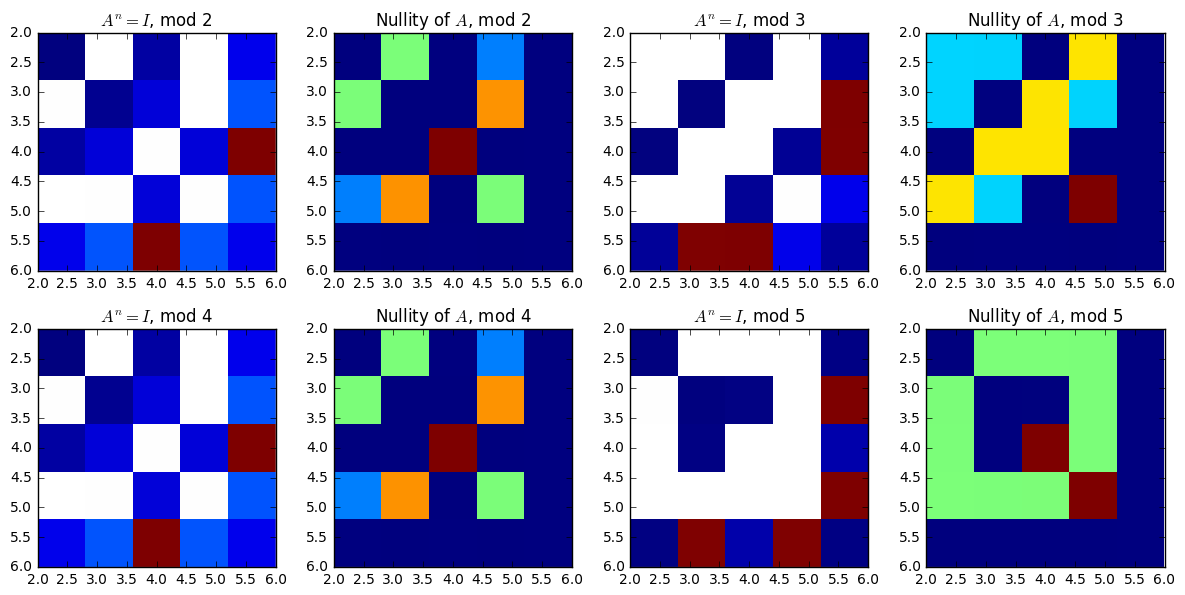
\includegraphics[width=\textwidth]{cycles-vs-nullity-small.png}
\end{figure}

\begin{figure}
  \caption{3-state transient path ending in a 6-state cycle of $A$ for \modZ{6} on a $5 \times 5$ grid.}
  \label{655-transient}
  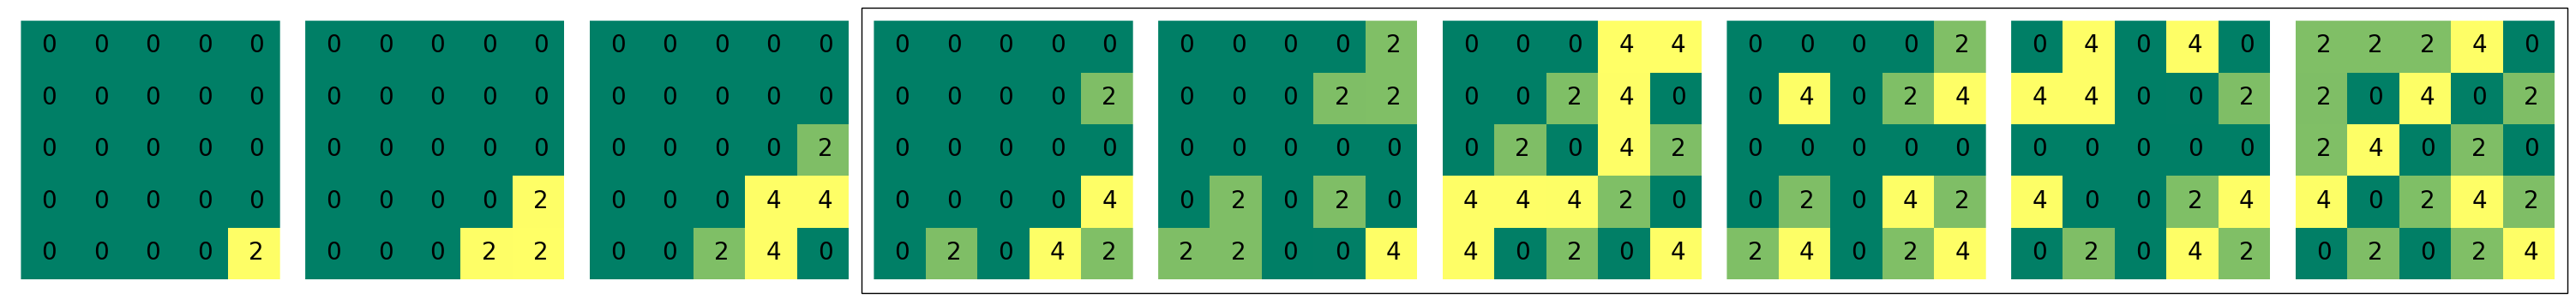
\includegraphics[width=\textwidth]{655-transient.png}
\end{figure}

\begin{figure}
  \caption{4-state transient path ending in a 12-state cycle of $A$ for \modZ{6} on a $5 \times 5$ grid.}
  \label{655-transient-long}
  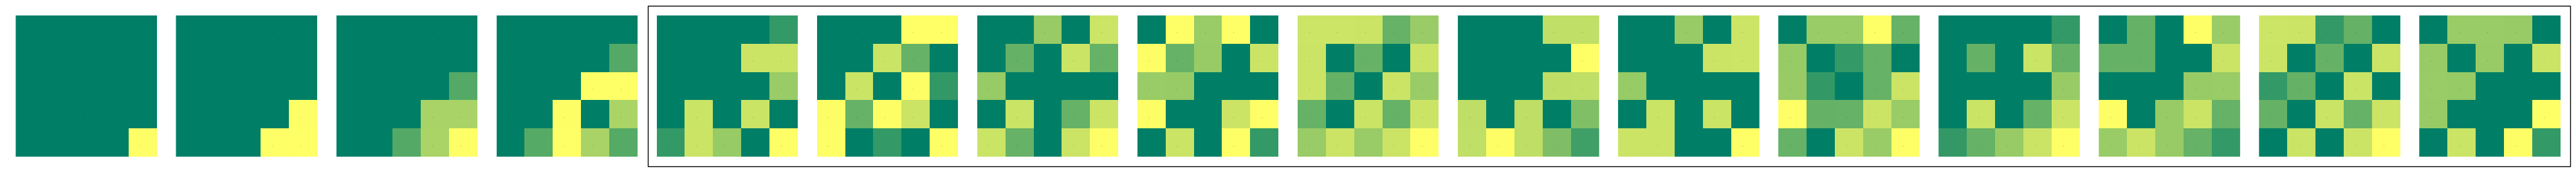
\includegraphics[width=\textwidth]{655-transient-long.png}
\end{figure}

\begin{figure}
  \caption{One of many intermediate frames from a solution video to a $64 \times 64$ grid in \modZ{51} with a complicated transition matrix $A_c$. Note that since $A_c$ is invertible, the sequence of presses on the right can be transformed back into the original image, which may be of interest cryptographically.}
  \label{chr-solution}
  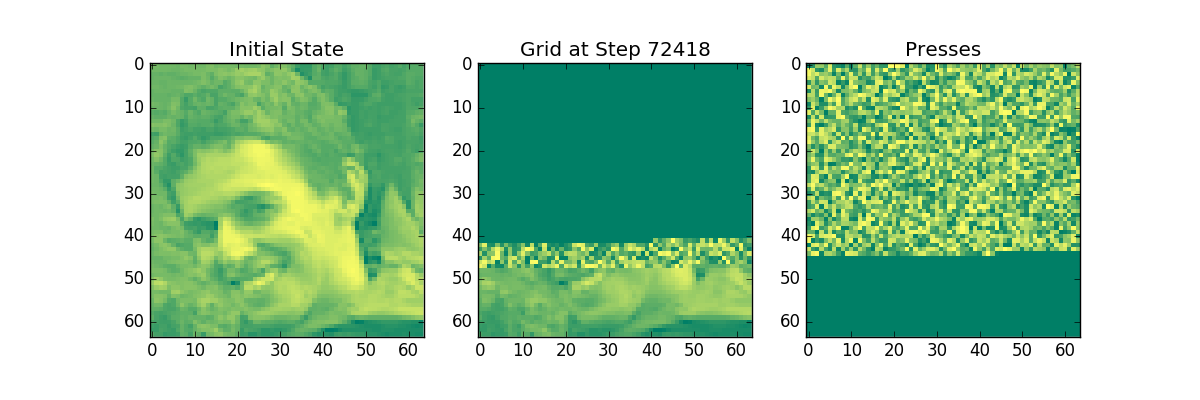
\includegraphics[width=\textwidth]{img000072418.png}
\end{figure}

\section*{Visually Appealing Solutions}

\clearpage

\begin{thebibliography}{9}
\bibitem{jaap}
  J. Scherphuis, \textit{The Mathematics of Lights Out},
  \href{http://www.jaapsch.net/puzzles/lomath.htm}{http://www.jaapsch.net/puzzles/lomath.htm}.
  Accessed December 2016.
\bibitem{giffen}
  A. Giffen and D. B. Parker, \textit{On Generalizing the "Lights Out" Game and a Generalization of Parity Domination}, preprint, 2009. Available at \href{http://faculty.gvsu.edu/parkerda/profstuff/papers/hyperlogpd.pdf}{http://faculty.gvsu.edu/parkerda/profstuff/papers/hyperlogpd.pdflink}.
\bibitem{involve}
  S. Edwards, V. Elandt, N. James, K. Johnson, Z. Mitchell, and D. Stephenson, \textit{Lights Out on finite graphs}, Involve 3 (2010), 17-32. Available at \href{http://msp.org/involve/2010/3-1/involve-v3-n1-p03-s.pdf}{http://msp.org/involve/2010/3-1/involve-v3-n1-p03-s.pdf}.
\end{thebibliography}

\end{document}
